\documentclass[tikz,border=2pt]{standalone}
\renewcommand{\familydefault}{\sfdefault}
\usetikzlibrary{arrows.meta,calc,positioning}
\tikzset{every picture/.style={line width=1pt, >=Stealth},
         hl/.style={fill=black, fill opacity=0.12, text opacity=1}}
\begin{document}
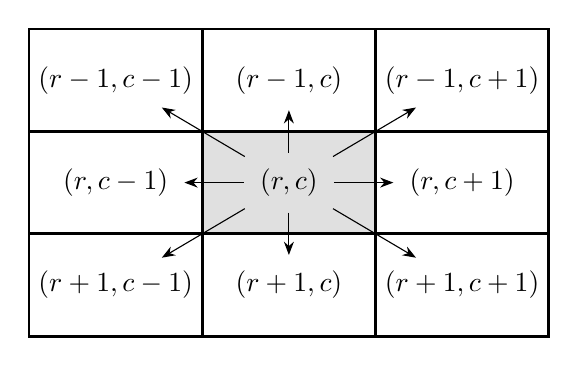
\begin{tikzpicture}[x=2.2cm, y=1.3cm, cell/.style={draw, minimum width=2.2cm, minimum height=1.3cm}]
  % Row r grows downward and column c grows rightward, as in the direction vectors.
  \foreach \r in {-1, 0, 1} \foreach \c in {-1, 0, 1} \node[cell] at (\c, -\r) {};
  \node[cell, hl] at (0, 0) {};
  \node (center) at (0, 0) {$(r, c)$};
  \foreach \dr/\dc/\label in {-1/0/{$(r-1, c)$}, 1/0/{$(r+1, c)$}, 0/-1/{$(r, c-1)$}, 0/1/{$(r, c+1)$}, -1/-1/{$(r-1, c-1)$}, -1/1/{$(r-1, c+1)$}, 1/1/{$(r+1, c+1)$}, 1/-1/{$(r+1, c-1)$}} {
    \node (n) at (\dc, -\dr) {\label};
    \draw[->, thin, shorten <=2pt, shorten >=2pt] (center) -- (n);
  }
\end{tikzpicture}
\end{document}
